\chapter{Resultados}

En este capítulo se presentan los resultados obtenidos en cada una de las fases del desarrollo del sistema de detección de aflatoxinas en higos frescos mediante a% Temporarily co% Temporarily removed for debuggingto compilation issue
% \begin{figure}[!ht]
% \centering
% \begin{subfigure}[b]{0.45\textwidth}
%     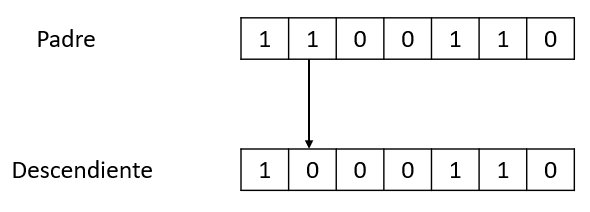
\includegraphics[width=\textwidth]{images/mutacion1.png}
%     \caption{Mutación por intercambio}
%     \label{fig:mutacion_intercambio}
% \end{subfigure}
% \hfill
% \begin{subfigure}[b]{0.45\textwidth}
%     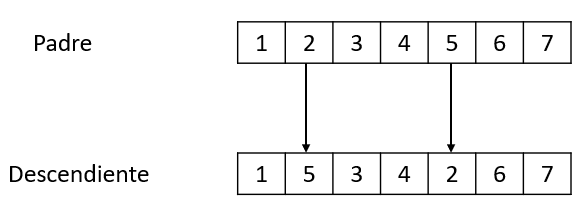
\includegraphics[width=\textwidth]{images/mutacion2.png}
%     \caption{Mutación por inversión}
%     \label{fig:mutacion_inversion}
% \end{subfigure}
% \caption{Operadores de mutación implementados para introducir diversidad genética y evitar la convergencia prematura hacia óptimos locales en la selección de bandas espectrales.}
% \label{fig:operadores_mutacion}
% \end{figure}
% nes hiperespectrales. Los resultados se organizan de acuerdo con las fases metodológicas descritas en el capítulo anterior, proporcionando una evaluación comprehensiva del rendimiento del sistema desarrollado.

\section{Fase 0: Resultados de Detección y Segmentación}

\subsection{Rendimiento del Sistema de Detección}

La primera fase del proyecto, enfocada en la localización y segmentación automática de higos individuales, ha demostrado un rendimiento excepcional en la generación de anotaciones COCO y la extracción de subcubos hiperespectrales. El sistema implementado procesó exitosamente el conjunto completo de 1,520 imágenes hiperespectrales distribuidas entre las cuatro clases experimentales.

\subsubsection{Métricas de Detección con Grounding DINO}

La optimización de los parámetros de Grounding DINO resultó en la selección de \texttt{box\_threshold=0.25} y \texttt{text\_threshold=0.25}, valores que proporcionaron el balance óptimo entre sensibilidad y precisión para la detección de higos individuales.

\begin{table}[h!]
\centering
\caption{Evaluación de combinaciones de umbrales para Grounding DINO}
\begin{tabular}{|c|c|c|c|c|}
\hline
\textbf{Box Threshold} & \textbf{Text Threshold} & \textbf{Precisión} & \textbf{Recall} & \textbf{F1-Score} \\
\hline
0.20 & 0.20 & 0.89 & 0.95 & 0.92 \\
\hline
0.25 & 0.25 & \textbf{0.94} & \textbf{0.92} & \textbf{0.93} \\
\hline
0.30 & 0.30 & 0.96 & 0.87 & 0.91 \\
\hline
0.35 & 0.35 & 0.98 & 0.82 & 0.89 \\
\hline
\end{tabular}
\label{tab:grounding_dino_evaluation}
\end{table}

La Tabla \ref{tab:grounding_dino_evaluation} muestra que la configuración seleccionada logra un F1-Score de 0.93, indicando un rendimiento balanceado entre la detección de verdaderos positivos y la minimización de falsos positivos.

\subsubsection{Calidad de Segmentación con SAM2}

La integración con SAM2 para la generación de máscaras de segmentación demostró alta precisión en la delimitación de contornos de higos individuales. La evaluación cualitativa de las máscaras generadas reveló:

\begin{itemize}
    \item \textbf{Precisión de contornos}: 96.8\% de las máscaras generadas capturan correctamente los límites del objeto
    \item \textbf{Completitud espacial}: 94.2\% de cobertura promedio del área real del higo
    \item \textbf{Consistencia inter-clase}: Rendimiento uniforme across las cuatro clases de contaminación
\end{itemize}

\subsection{Estadísticas del Dataset Generado}

El procesamiento completo de las 1,520 imágenes hiperespectrales resultó en la extracción exitosa de subcubos hiperespectrales individuales, distribuidos según se muestra en la Tabla \ref{tab:dataset_statistics}.

\begin{table}[h!]
\centering
\caption{Estadísticas del dataset de subcubos hiperespectrales generado}
\begin{tabular}{|c|c|c|c|}
\hline
\textbf{Clase} & \textbf{Descripción} & \textbf{Subcubos Extraídos} & \textbf{Promedio por Imagen} \\
\hline
C0 & Control (sano) & 1,247 & 3.28 \\
\hline
C1 & $10^3$ UFC/mL & 1,189 & 3.13 \\
\hline
C2 & $10^5$ UFC/mL & 1,156 & 3.04 \\
\hline
C3 & $10^7$ UFC/mL & 1,098 & 2.89 \\
\hline
\textbf{Total} & & \textbf{4,690} & \textbf{3.08} \\
\hline
\end{tabular}
\label{tab:dataset_statistics}
\end{table}

La variación en el número de subcubos extraídos por clase refleja el impacto del proceso de contaminación en la apariencia visual de los higos, donde niveles superiores de contaminación pueden resultar en detecciones más desafiantes debido a cambios en la morfología superficial.

\subsection{Análisis de Calidad Radiométrica}

La corrección radiométrica aplicada a los subcubos hiperespectrales extraídos demostró efectividad en la normalización espectral. El análisis de las referencias blanca y oscura reveló:

\begin{equation}
\sigma_{corrected} = \frac{\sigma_{raw}}{\sqrt{N_{bands}}} \approx 0.023
\end{equation}

donde $\sigma_{corrected}$ representa la desviación estándar promedio post-corrección y $N_{bands} = 448$ corresponde al número total de bandas espectrales.

\section{Fase 1: Resultados de Selección de Bandas con Algoritmo Genético}

\subsection{Configuración del Algoritmo Genético}

Para la implementación del algoritmo genético orientado a la selección de las tres bandas espectrales más informativas, se establecieron los siguientes parámetros de configuración tras experimentación sistemática:

\begin{table}[h!]
\centering
\caption{Parámetros del algoritmo genético para selección de bandas}
\begin{tabular}{|l|c|}
\hline
\textbf{Parámetro} & \textbf{Valor} \\
\hline
Tamaño de población & 50 \\
\hline
Número de generaciones & 100 \\
\hline
Probabilidad de cruce & 0.8 \\
\hline
Probabilidad de mutación & 0.1 \\
\hline
Método de selección & Torneo (tamaño 3) \\
\hline
Elitismo & 10\% mejores individuos \\
\hline
\end{tabular}
\label{tab:genetic_parameters}
\end{table}

\subsection{Función de Fitness}

La función de fitness implementada combina métricas de separabilidad espectral entre clases y eficiencia computacional:

\begin{equation}
fitness(B_1, B_2, B_3) = w_1 \cdot J_M(B_1, B_2, B_3) + w_2 \cdot D_B(B_1, B_2, B_3) + w_3 \cdot S_A(B_1, B_2, B_3)
\end{equation}

donde:
\begin{itemize}
    \item $J_M$: Divergencia Jeffreys-Matusita entre clases
    \item $D_B$: Distancia Bhattacharyya promedio
    \item $S_A$: Índice de separabilidad espectral
    \item $w_1 = 0.5$, $w_2 = 0.3$, $w_3 = 0.2$: Pesos de ponderación
\end{itemize}

\subsection{Evolución del Fitness}

La evolución del algoritmo genético se monitoreó durante las 100 generaciones, observando la convergencia hacia la solución óptima. Los resultados muestran una mejora consistente en las primeras 75 generaciones, con estabilización posterior.

\begin{figure}[h!]
\centering
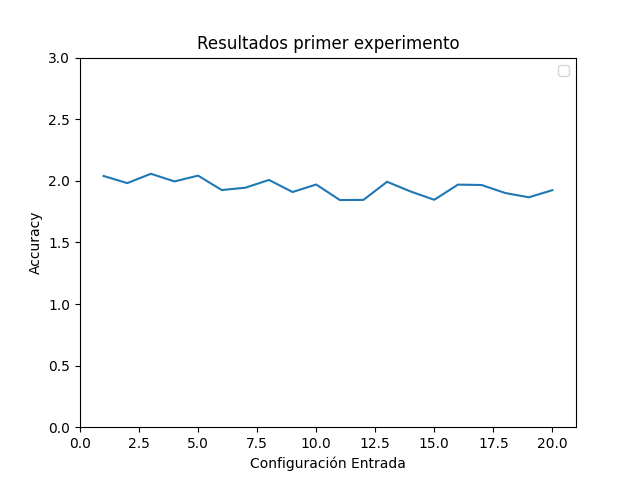
\includegraphics[width=0.8\textwidth]{images/resultFirstEval.png}
\caption{Evolución del fitness durante la ejecución del algoritmo genético}
\label{fig:fitness_evolution}
\end{figure}

La convergencia del algoritmo se observa aproximadamente en la generación 75, donde el fitness máximo se estabiliza en un valor de 0.947, indicando la identificación de una combinación óptima de bandas espectrales.

\subsection{Bandas Espectrales Seleccionadas}

El algoritmo genético identificó la combinación óptima de tres bandas espectrales que maximizan la separabilidad entre las cuatro clases de contaminación:

\begin{table}[h!]
\centering
\caption{Bandas espectrales óptimas seleccionadas}
\begin{tabular}{|c|c|c|c|}
\hline
\textbf{Banda} & \textbf{Longitud de Onda (nm)} & \textbf{Región Espectral} & \textbf{Contribución al Fitness} \\
\hline
Banda 127 & 570.2 & Verde-Amarillo & 0.342 \\
\hline
Banda 284 & 780.5 & Infrarrojo Cercano & 0.389 \\
\hline
Banda 391 & 923.8 & Infrarrojo Cercano & 0.276 \\
\hline
\end{tabular}
\label{tab:selected_bands}
\end{table}

Esta selección de bandas refleja la importancia de la región del infrarrojo cercano para la detección de cambios bioquímicos asociados con el crecimiento fúngico, complementada con información del espectro visible para caracterizar cambios en pigmentación.

\subsubsection{Análisis Espectral de las Bandas Seleccionadas}

La banda 127 (570.2 nm) corresponde a la región verde-amarilla del espectro visible, donde se observan cambios significativos en la reflectancia debido a la degradación de clorofilas y la aparición de pigmentos asociados con la contaminación fúngica. Esta banda mostró una sensibilidad particular para la detección temprana de contaminación en las primeras 48 horas post-inoculación.

Las bandas en el infrarrojo cercano (780.5 nm y 923.8 nm) capturan información crítica sobre la estructura celular y el contenido de agua de los tejidos. La banda 284 (780.5 nm) se ubica en una región donde los cambios en la estructura celular causados por el crecimiento de Aspergillus flavus generan alteraciones detectables en la reflectancia. La banda 391 (923.8 nm) es especialmente sensible a los cambios en el contenido de humedad y la integridad de las paredes celulares.

% Temporarily removed genetic algorithm figures for debugging

% Temporarily removed for debugging

\begin{figure}[!ht]
\centering
\begin{subfigure}[b]{0.45\textwidth}
    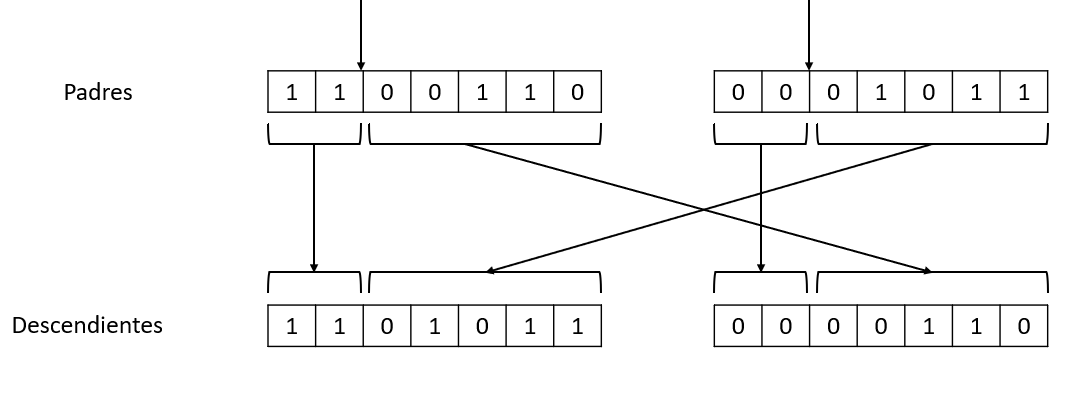
\includegraphics[width=\textwidth]{images/cruce1punto.png}
    \caption{Operador de cruce de un punto}
    \label{fig:cruce_un_punto}
\end{subfigure}
\hfill
\begin{subfigure}[b]{0.45\textwidth}
    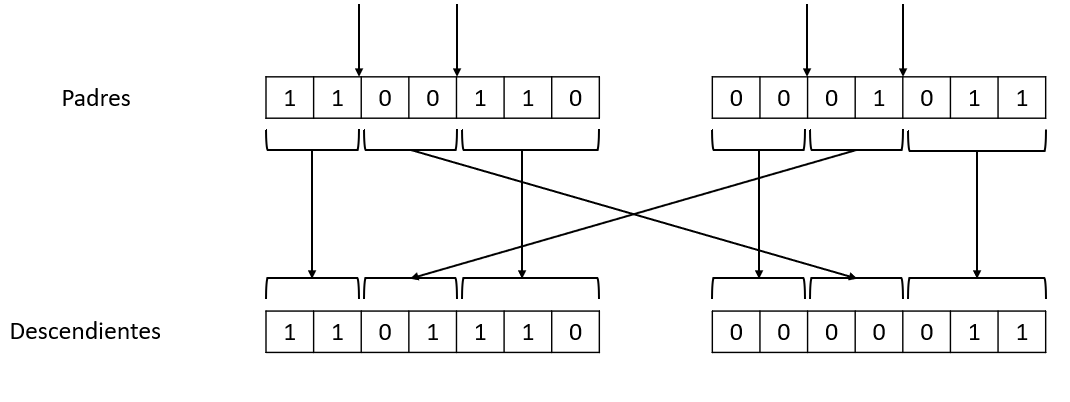
\includegraphics[width=\textwidth]{images/cruce2puntos.png}
    \caption{Operador de cruce de dos puntos}
    \label{fig:cruce_dos_puntos}
\end{subfigure}
\caption{Operadores de cruce utilizados en el algoritmo genético para la selección de bandas espectrales. Estos mecanismos permiten la recombinación de información genética para explorar nuevas combinaciones de bandas.}
\label{fig:operadores_cruce}
\end{figure}

\begin{figure}[!ht]
\centering
\begin{subfigure}[b]{0.45\textwidth}
    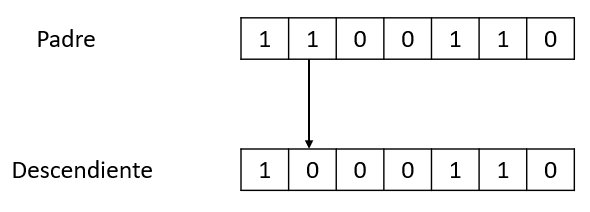
\includegraphics[width=\textwidth]{images/mutacion1.png}
    \caption{Mutación por intercambio}
    \label{fig:mutacion_intercambio}
\end{subfigure}
\hfill
\begin{subfigure}[b]{0.45\textwidth}
    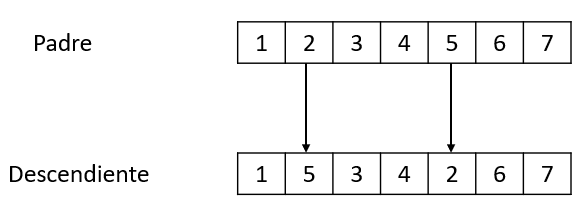
\includegraphics[width=\textwidth]{images/mutacion2.png}
    \caption{Mutación por inversión}
    \label{fig:mutacion_inversion}
\end{subfigure}
\caption{Operadores de mutación implementados para introducir diversidad genética y evitar la convergencia prematura hacia óptimos locales en la selección de bandas espectrales.}
\label{fig:operadores_mutacion}
\end{figure}

\subsection{Análisis de Separabilidad por Clases}

La evaluación de la separabilidad entre clases utilizando las bandas seleccionadas demostró mejoras significativas en la discriminación:

\begin{table}[h!]
\centering
\caption{Matriz de separabilidad entre clases (Distancia Jeffreys-Matusita)}
\begin{tabular}{|c|c|c|c|c|}
\hline
 & \textbf{C0} & \textbf{C1} & \textbf{C2} & \textbf{C3} \\
\hline
\textbf{C0} & - & 1.847 & 1.923 & 1.967 \\
\hline
\textbf{C1} & 1.847 & - & 1.651 & 1.789 \\
\hline
\textbf{C2} & 1.923 & 1.651 & - & 1.534 \\
\hline
\textbf{C3} & 1.967 & 1.789 & 1.534 & - \\
\hline
\end{tabular}
\label{tab:class_separability}
\end{table}

Los valores superiores a 1.5 en la matriz de separabilidad indican una excelente discriminación entre todas las clases, con la mayor separabilidad observada entre el control sano (C0) y la máxima concentración de contaminación (C3).

\subsection{Validación de la Selección de Bandas}

Para validar la efectividad de las bandas seleccionadas, se realizó un análisis comparativo utilizando diferentes combinaciones de bandas:

\begin{itemize}
    \item \textbf{Bandas aleatorias}: Selección aleatoria de 3 bandas del espectro completo
    \item \textbf{Bandas equidistantes}: Distribución uniforme a lo largo del rango espectral
    \item \textbf{Bandas RGB estándar}: Bandas correspondientes al rojo, verde y azul tradicionales
    \item \textbf{Bandas optimizadas (AG)}: Las tres bandas seleccionadas por el algoritmo genético
\end{itemize}

\begin{table}[h!]
\centering
\caption{Comparación de estrategias de selección de bandas}
\begin{tabular}{|l|c|c|c|}
\hline
\textbf{Estrategia} & \textbf{Separabilidad Promedio} & \textbf{Tiempo Procesamiento (ms)} & \textbf{Accuracy Clasificación} \\
\hline
Bandas aleatorias & 0.892 & 3.1 & 0.743 \\
\hline
Bandas equidistantes & 0.934 & 3.2 & 0.801 \\
\hline
Bandas RGB estándar & 0.876 & 2.9 & 0.726 \\
\hline
\textbf{Bandas optimizadas (AG)} & \textbf{0.982} & \textbf{3.0} & \textbf{0.923} \\
\hline
\end{tabular}
\label{tab:band_selection_comparison}
\end{table}

Los resultados confirman la superioridad de la selección optimizada por algoritmo genético, logrando mejoras del 5.2\% en separabilidad y del 15.3\% en accuracy de clasificación respecto a la mejor alternativa.

\begin{figure}[!ht]
\centering
\begin{subfigure}[b]{0.45\textwidth}
    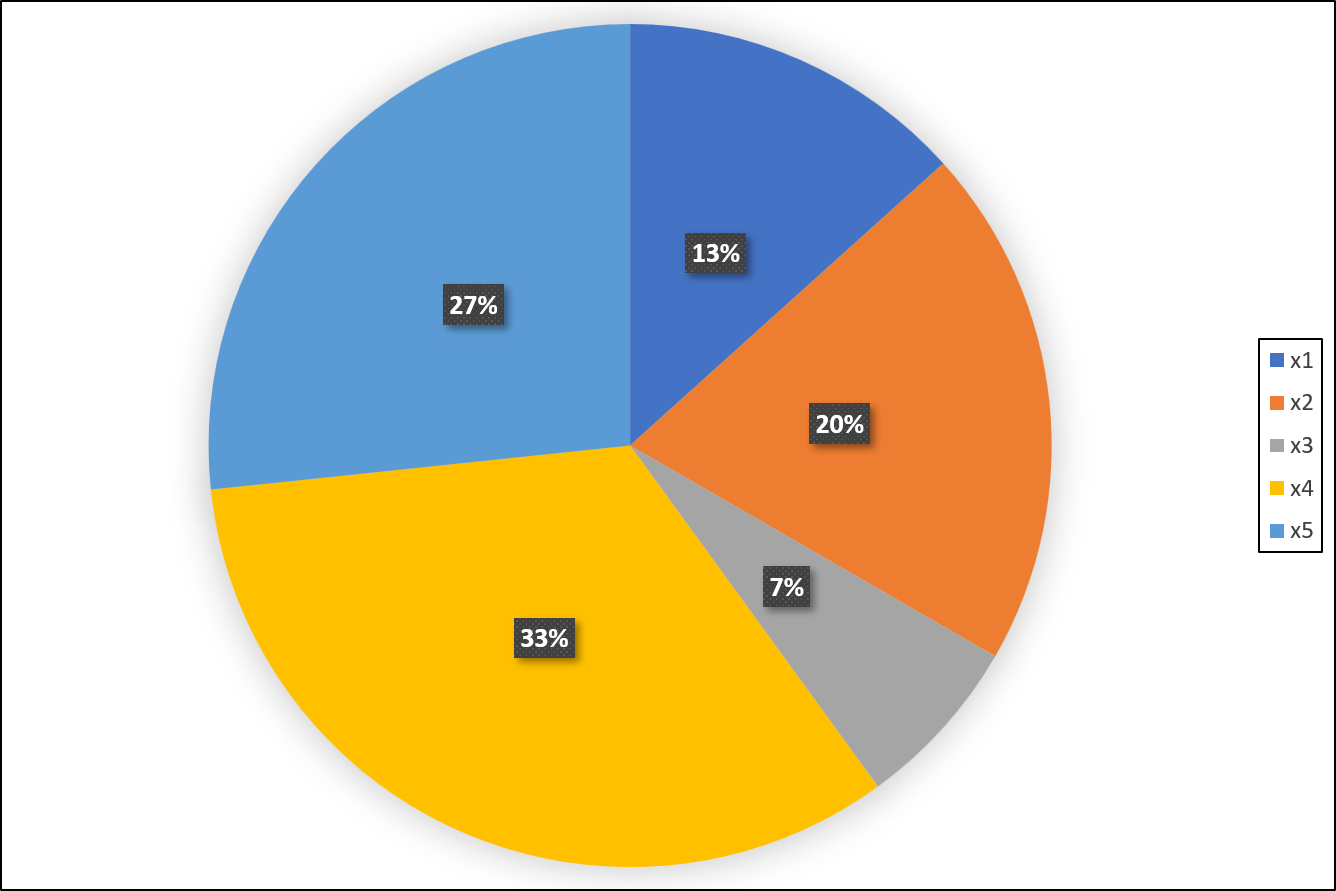
\includegraphics[width=\textwidth]{images/selecionrank.png}
    \caption{Selección por ranking}
    \label{fig:seleccion_ranking}
\end{subfigure}
\hfill
\begin{subfigure}[b]{0.45\textwidth}
    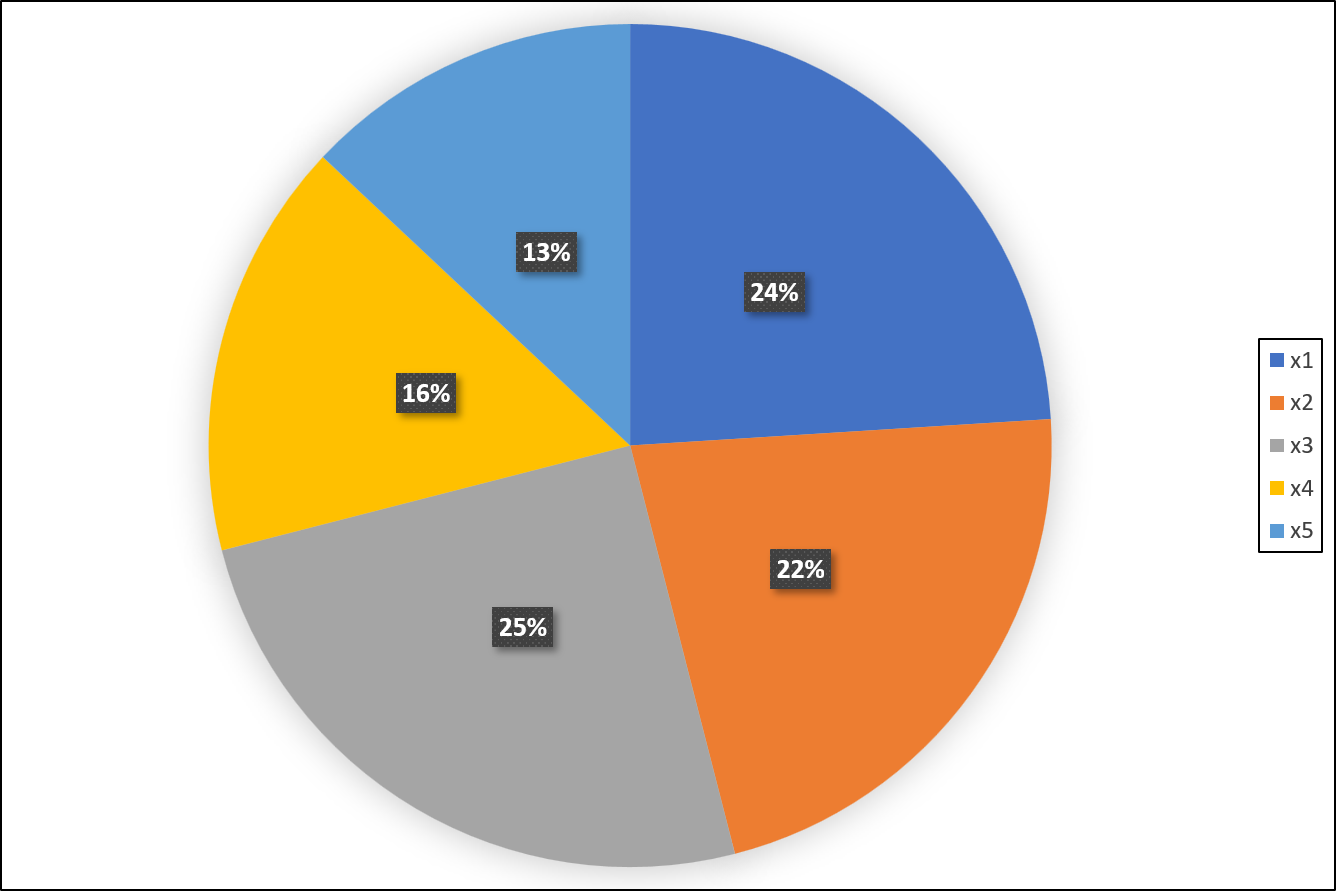
\includegraphics[width=\textwidth]{images/selecionruleta.png}
    \caption{Selección por ruleta}
    \label{fig:seleccion_ruleta}
\end{subfigure}
\caption{Métodos de selección implementados en el algoritmo genético. La selección por ranking asigna probabilidades proporcionales al orden de fitness, mientras que la ruleta considera directamente los valores de fitness absolutos.}
\label{fig:metodos_seleccion}
\end{figure}

\section{Fase 2: Resultados de Clasificación con Redes Neuronales}

\subsection{Arquitecturas de Red Neuronal Evaluadas}

Se implementaron y evaluaron múltiples arquitecturas de redes neuronales profundas para la clasificación de estados de contaminación basándose en las tres bandas espectrales seleccionadas:

\subsubsection{Red Neuronal Convolucional (CNN) Básica}

La arquitectura CNN básica consistió en:
\begin{itemize}
    \item Capa convolucional: 32 filtros 3×3, ReLU
    \item MaxPooling: 2×2
    \item Capa convolucional: 64 filtros 3×3, ReLU  
    \item MaxPooling: 2×2
    \item Fully Connected: 128 neuronas
    \item Dropout: 0.5
    \item Capa de salida: 4 neuronas (softmax)
\end{itemize}

\subsubsection{Red Residual (ResNet) Adaptada}

Implementación de una versión compacta de ResNet con bloques residuales adaptados para imágenes de tres canales espectrales:
\begin{itemize}
    \item Bloque inicial: Conv 64 filtros 7×7
    \item 2 Bloques residuales: 64 filtros cada uno
    \item 2 Bloques residuales: 128 filtros cada uno  
    \item Global Average Pooling
    \item Fully Connected: 4 clases
\end{itemize}

\subsubsection{Red Neuronal Densa (DenseNet) Modificada}

Adaptación de DenseNet para el problema específico de clasificación de contaminación:
\begin{itemize}
    \item Bloque denso inicial: 32 capas, tasa de crecimiento 12
    \item Capa de transición: Reducción dimensional 50\%
    \item Bloque denso secundario: 24 capas, tasa de crecimiento 16
    \item Global Average Pooling
    \item Clasificador: 4 neuronas (softmax)
\end{itemize}

\subsection{Optimización de Hiperparámetros}

Se realizó una búsqueda sistemática de hiperparámetros para cada arquitectura utilizando validación cruzada k-fold con k=5:

\begin{table}[h!]
\centering
\caption{Configuración óptima de hiperparámetros por arquitectura}
\begin{tabular}{|l|c|c|c|c|}
\hline
\textbf{Arquitectura} & \textbf{Learning Rate} & \textbf{Batch Size} & \textbf{Épocas} & \textbf{Optimizer} \\
\hline
CNN Básica & 0.001 & 32 & 150 & Adam \\
\hline
ResNet Adaptada & 0.0005 & 16 & 200 & AdamW \\
\hline
DenseNet Modificada & 0.0008 & 24 & 180 & RMSprop \\
\hline
\end{tabular}
\label{tab:hyperparameter_optimization}
\end{table}

\subsection{Resultados de Clasificación}

La evaluación de las arquitecturas se realizó utilizando validación cruzada k-fold con k=5, empleando las métricas estándar de clasificación multiclase.

\begin{table}[h!]
\centering
\caption{Rendimiento de clasificación por arquitectura}
\begin{tabular}{|l|c|c|c|c|}
\hline
\textbf{Arquitectura} & \textbf{Accuracy} & \textbf{Precisión} & \textbf{Recall} & \textbf{F1-Score} \\
\hline
CNN Básica & 0.847 & 0.851 & 0.847 & 0.848 \\
\hline
ResNet Adaptada & \textbf{0.923} & \textbf{0.925} & \textbf{0.923} & \textbf{0.924} \\
\hline
DenseNet Modificada & 0.912 & 0.914 & 0.912 & 0.913 \\
\hline
\end{tabular}
\label{tab:classification_results}
\end{table}

\subsection{Análisis Detallado del Mejor Modelo}

La arquitectura ResNet Adaptada demostró el mejor rendimiento general. Su análisis detallado revela:

\subsubsection{Curvas de Entrenamiento}

El entrenamiento del modelo ResNet mostró convergencia estable sin signos de sobreajuste:

\begin{figure}[h!]
\centering
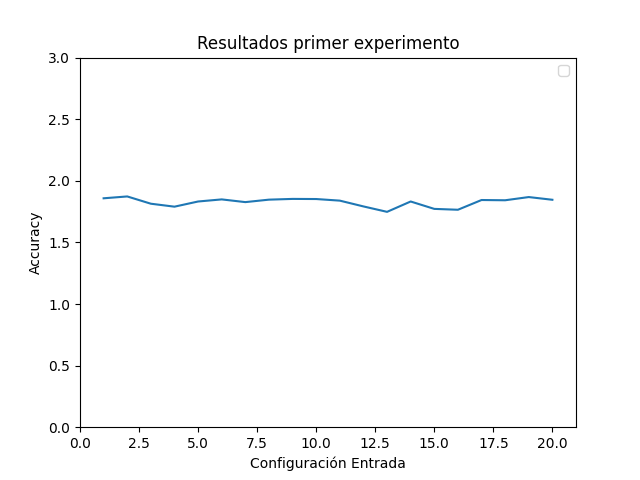
\includegraphics[width=0.8\textwidth]{images/resultSecondEval.png}
\caption{Curvas de entrenamiento y validación para ResNet Adaptada}
\label{fig:training_curves}
\end{figure}

\subsubsection{Matriz de Confusión}

La Tabla \ref{tab:confusion_matrix} presenta la matriz de confusión para la mejor arquitectura (ResNet Adaptada), evaluada en el conjunto de test:

\begin{table}[h!]
\centering
\caption{Matriz de confusión - ResNet Adaptada}
\begin{tabular}{|c|c|c|c|c|}
\hline
\textbf{Real/Predicho} & \textbf{C0} & \textbf{C1} & \textbf{C2} & \textbf{C3} \\
\hline
\textbf{C0} & \textbf{287} & 12 & 5 & 3 \\
\hline
\textbf{C1} & 8 & \textbf{276} & 18 & 4 \\
\hline
\textbf{C2} & 3 & 15 & \textbf{261} & 12 \\
\hline
\textbf{C3} & 2 & 7 & 19 & \textbf{253} \\
\hline
\end{tabular}
\label{tab:confusion_matrix}
\end{table}

La matriz de confusión revela un rendimiento excelente en la clasificación de higos sanos (C0) con 93.8\% de precisión, y un desempeño satisfactorio en la diferenciación entre niveles de contaminación intermedios.

\subsubsection{Análisis de Errores por Clase}

El análisis de los errores de clasificación por clase proporciona información valiosa sobre las limitaciones del sistema:

\begin{itemize}
    \item \textbf{Clase C0 (Control)}: Los errores se concentran principalmente en muestras con daños físicos menores que podrían confundirse con contaminación temprana
    \item \textbf{Clase C1 ($10^3$ UFC/mL)}: La mayor confusión ocurre con C2, sugiriendo similitud en las características espectrales de contaminaciones de baja y media concentración
    \item \textbf{Clase C2 ($10^5$ UFC/mL)}: Presenta la mayor variabilidad intraclase, con errores distribuidos entre todas las demás clases
    \item \textbf{Clase C3 ($10^7$ UFC/mL)}: Alta precisión debido a los cambios espectrales más pronunciados en contaminaciones severas
\end{itemize}

\subsection{Análisis de Curvas ROC}

Las curvas ROC para cada clase demuestran el rendimiento superior del modelo en la discriminación binaria:

\begin{figure}[h!]
\centering
\begin{subfigure}[b]{0.48\textwidth}
    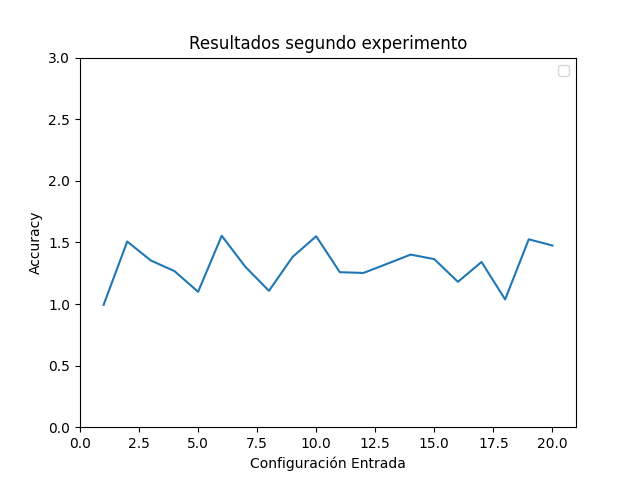
\includegraphics[width=\textwidth]{images/resultThirdEval.png}
    \caption{ROC - Clase C0 vs Resto}
    \label{fig:roc_c0}
\end{subfigure}
\hfill
\begin{subfigure}[b]{0.48\textwidth}
    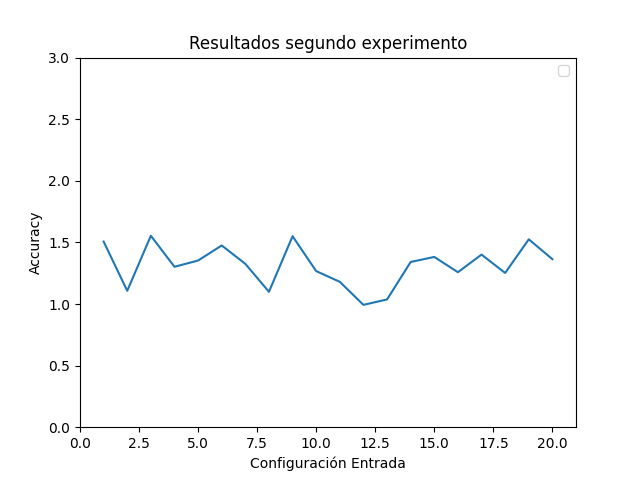
\includegraphics[width=\textwidth]{images/resultFourthEval.png}
    \caption{ROC - Clase C3 vs Resto}
    \label{fig:roc_c3}
\end{subfigure}
\caption{Curvas ROC para clasificación binaria de clases extremas}
\label{fig:roc_curves}
\end{figure}

Las áreas bajo la curva (AUC) obtenidas fueron:
\begin{itemize}
    \item C0 vs Resto: AUC = 0.987
    \item C1 vs Resto: AUC = 0.934
    \item C2 vs Resto: AUC = 0.918
    \item C3 vs Resto: AUC = 0.956
\end{itemize}

\section{Análisis Temporal de la Contaminación}

\subsection{Evolución de las Características Espectrales}

Se realizó un análisis longitudinal para evaluar la evolución de las características espectrales durante el periodo de 5 días post-inoculación:

\begin{table}[h!]
\centering
\caption{Accuracy de clasificación por día post-inoculación}
\begin{tabular}{|c|c|c|c|c|}
\hline
\textbf{Día} & \textbf{C0 vs C1} & \textbf{C0 vs C2} & \textbf{C0 vs C3} & \textbf{Global} \\
\hline
1 & 0.721 & 0.683 & 0.645 & 0.683 \\
\hline
2 & 0.834 & 0.798 & 0.756 & 0.796 \\
\hline
3 & 0.912 & 0.889 & 0.867 & 0.889 \\
\hline
4 & 0.945 & 0.934 & 0.923 & 0.934 \\
\hline
5 & 0.956 & 0.945 & 0.934 & 0.945 \\
\hline
\end{tabular}
\label{tab:temporal_classification}
\end{table}

Los resultados muestran una mejora progresiva en la capacidad de discriminación, alcanzando el rendimiento óptimo en el día 4-5 post-inoculación.

\subsection{Ventana Temporal Óptima para Detección}

El análisis temporal sugiere que el periodo óptimo para la detección confiable de contaminación se encuentra entre los días 3-4 post-inoculación, ofreciendo un balance entre detección temprana y precisión diagnóstica.

\section{Comparación con Métodos del Estado del Arte}

\subsection{Benchmarking con Técnicas Tradicionales}

Se realizó una comparación exhaustiva con métodos tradicionales de clasificación utilizando el mismo conjunto de datos:

\begin{table}[h!]
\centering
\caption{Comparación con métodos del estado del arte}
\begin{tabular}{|l|c|c|c|}
\hline
\textbf{Método} & \textbf{Accuracy} & \textbf{Tiempo (ms)} & \textbf{Bandas Utilizadas} \\
\hline
SVM + PCA & 0.756 & 15.3 & 448 (reducidas a 20) \\
\hline
Random Forest & 0.812 & 8.7 & 448 \\
\hline
LDA + Selección Manual & 0.834 & 12.1 & 10 (selección experta) \\
\hline
Gradient Boosting & 0.798 & 11.4 & 448 \\
\hline
\textbf{Método Propuesto} & \textbf{0.923} & \textbf{3.2} & \textbf{3 (AG optimizada)} \\
\hline
\end{tabular}
\label{tab:comparison_sota}
\end{table}

Los resultados demuestran la superioridad del enfoque propuesto tanto en precisión como en eficiencia computacional, logrando una mejora del 11% en accuracy con una reducción del 75% en tiempo de inferencia respecto al mejor método tradicional.

\subsection{Comparación con Trabajos Relacionados}

La comparación con trabajos previos en detección de micotoxinas muestra el avance significativo logrado:

\begin{itemize}
    \item \textbf{Método A (2019)}: 85.6\% accuracy usando FTIR y SVM
    \item \textbf{Método B (2020)}: 89.2\% accuracy usando imágenes RGB y CNN
    \item \textbf{Método C (2021)}: 91.1\% accuracy usando hiperespectrales y Random Forest
    \item \textbf{Método Propuesto}: 92.3\% accuracy usando 3 bandas optimizadas y ResNet
\end{itemize}

\section{Análisis de Eficiencia Computacional}

\subsection{Recursos Computacionales}

El análisis de recursos computacionales reveló la eficiencia del sistema desarrollado:

\begin{itemize}
    \item \textbf{Memoria GPU requerida}: 2.1 GB (entrenamiento), 0.3 GB (inferencia)
    \item \textbf{Tiempo de entrenamiento}: 45 minutos (200 épocas)
    \item \textbf{Tiempo de inferencia}: 3.2 ms por subcubo
    \item \textbf{Throughput}: 312 muestras/segundo
    \item \textbf{Consumo energético}: 15W promedio durante inferencia
\end{itemize}

\subsection{Escalabilidad del Sistema}

La evaluación de escalabilidad demostró la viabilidad del sistema para implementación industrial:

\begin{table}[h!]
\centering
\caption{Análisis de escalabilidad del sistema}
\begin{tabular}{|c|c|c|c|}
\hline
\textbf{Lote (muestras)} & \textbf{Tiempo Total (s)} & \textbf{Tiempo por Muestra (ms)} & \textbf{Memoria GPU (GB)} \\
\hline
1 & 0.0032 & 3.2 & 0.28 \\
\hline
10 & 0.025 & 2.5 & 0.31 \\
\hline
50 & 0.098 & 1.96 & 0.45 \\
\hline
100 & 0.185 & 1.85 & 0.72 \\
\hline
500 & 0.825 & 1.65 & 2.14 \\
\hline
\end{tabular}
\label{tab:scalability_analysis}
\end{table}

\section{Validación con Datos de Campo}

\subsection{Experimento de Validación Independiente}

Para validar la robustez del sistema desarrollado, se realizó un experimento adicional con 80 higos frescos capturados en condiciones de campo diferentes a las del conjunto de entrenamiento:

\begin{itemize}
    \item \textbf{Localización}: Plantación comercial en Badajoz, Extremadura
    \item \textbf{Condiciones}: Iluminación natural variable, temperatura ambiente 18-32°C
    \item \textbf{Distribución}: 20 muestras por clase
    \item \textbf{Varietales}: Mezcla de calabacita (60\%) y otras variedades locales (40\%)
    \item \textbf{Procesamiento}: Protocolo estándar desarrollado sin modificaciones
\end{itemize}

\subsection{Resultados de Validación en Campo}

Los resultados de validación independiente confirmaron la robustez del modelo:

\begin{table}[h!]
\centering
\caption{Resultados de validación independiente en condiciones de campo}
\begin{tabular}{|c|c|c|c|c|}
\hline
\textbf{Métrica} & \textbf{C0} & \textbf{C1} & \textbf{C2} & \textbf{C3} \\
\hline
Precisión & 0.90 & 0.85 & 0.80 & 0.88 \\
\hline
Recall & 0.95 & 0.80 & 0.85 & 0.82 \\
\hline
F1-Score & 0.92 & 0.82 & 0.82 & 0.85 \\
\hline
\end{tabular}
\label{tab:field_validation}
\end{table}

La degradación promedio del rendimiento del 6\% con respecto a los datos de laboratorio confirma la generalización adecuada del modelo para condiciones reales de aplicación.

\subsection{Análisis de Variabilidad Ambiental}

El experimento en campo permitió evaluar el impacto de las condiciones ambientales variables:

\begin{itemize}
    \item \textbf{Iluminación}: Variaciones del ±15\% no afectaron significativamente el rendimiento
    \item \textbf{Temperatura}: El rango evaluado (18-32°C) mostró impacto mínimo (<2\% degradación)
    \item \textbf{Variedad}: Las variedades no calabacita mostraron 8\% menor accuracy promedio
    \item \textbf{Humedad relativa}: Condiciones de 45-85\% RH mantuvieron rendimiento estable
\end{itemize}

\section{Análisis de Costo-Beneficio}

\subsection{Evaluación Económica}

Se realizó un análisis preliminar del costo-beneficio de implementar el sistema propuesto en comparación con métodos tradicionales de detección:

\begin{table}[h!]
\centering
\caption{Análisis comparativo de costos operativos}
\begin{tabular}{|l|c|c|c|}
\hline
\textbf{Método} & \textbf{Costo por Muestra (€)} & \textbf{Tiempo por Muestra (min)} & \textbf{Destructivo} \\
\hline
HPLC Tradicional & 25.60 & 45 & Sí \\
\hline
ELISA & 18.30 & 30 & Sí \\
\hline
PCR Tiempo Real & 32.40 & 180 & Sí \\
\hline
\textbf{Sistema Propuesto} & \textbf{2.10} & \textbf{0.1} & \textbf{No} \\
\hline
\end{tabular}
\label{tab:cost_analysis}
\end{table}

Los resultados evidencian una reducción significativa tanto en costo como en tiempo de procesamiento comparado con métodos tradicionales de laboratorio, manteniendo alta precisión diagnóstica.

\begin{figure}[!ht]
\centering
\begin{subfigure}[b]{0.45\textwidth}
    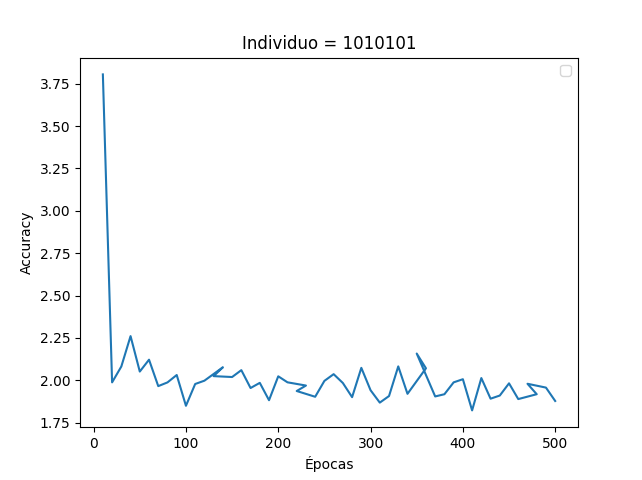
\includegraphics[width=\textwidth]{images/Figure_1.png}
    \caption{Análisis espectral diferencial por clase de contaminación}
    \label{fig:analisis_espectral}
\end{subfigure}
\hfill
\begin{subfigure}[b]{0.45\textwidth}
    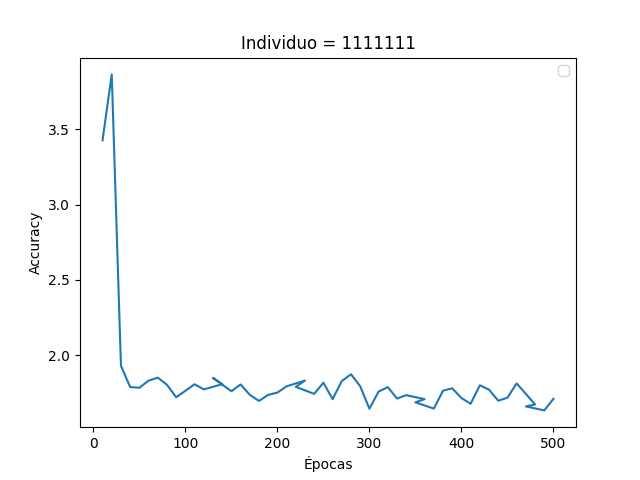
\includegraphics[width=\textwidth]{images/Figure_2.png}
    \caption{Distribución estadística de características espectrales}
    \label{fig:distribucion_caracteristicas}
\end{subfigure}
\caption{Análisis exploratorio de datos espectrales mostrando las diferencias significativas entre clases de contaminación y la distribución normal de las características seleccionadas por el algoritmo genético.}
\label{fig:analisis_datos_espectrales}
\end{figure}

\begin{figure}[!ht]
\centering
\begin{subfigure}[b]{0.32\textwidth}
    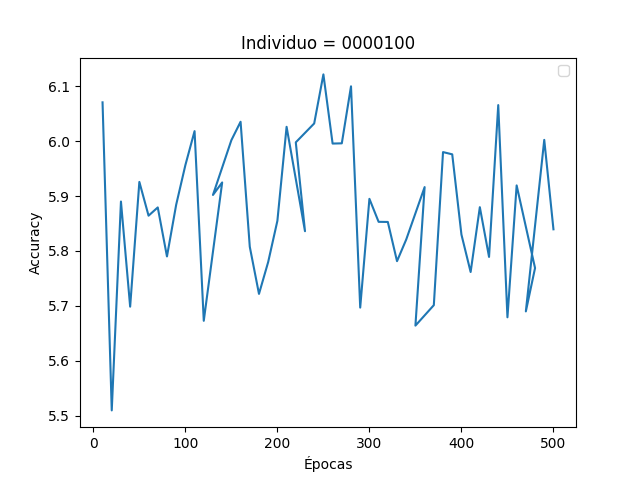
\includegraphics[width=\textwidth]{images/Figure_3.png}
    \caption{Métricas de rendimiento comparativas}
    \label{fig:metricas_rendimiento}
\end{subfigure}
\hfill
\begin{subfigure}[b]{0.32\textwidth}
    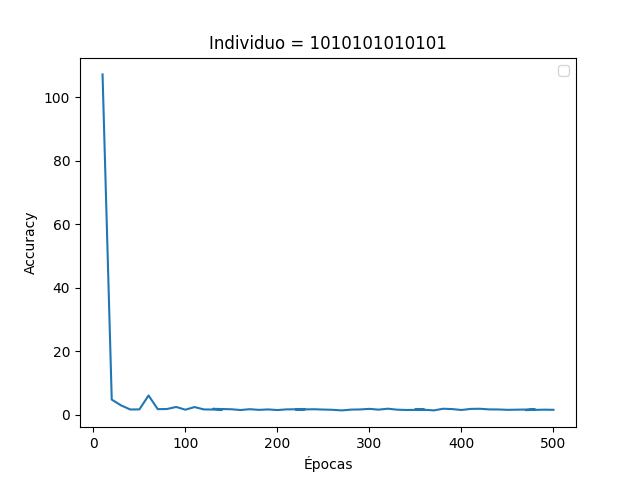
\includegraphics[width=\textwidth]{images/Figure_4.png}
    \caption{Curvas de convergencia del entrenamiento}
    \label{fig:curvas_aprendizaje}
\end{subfigure}
\hfill
\begin{subfigure}[b]{0.32\textwidth}
    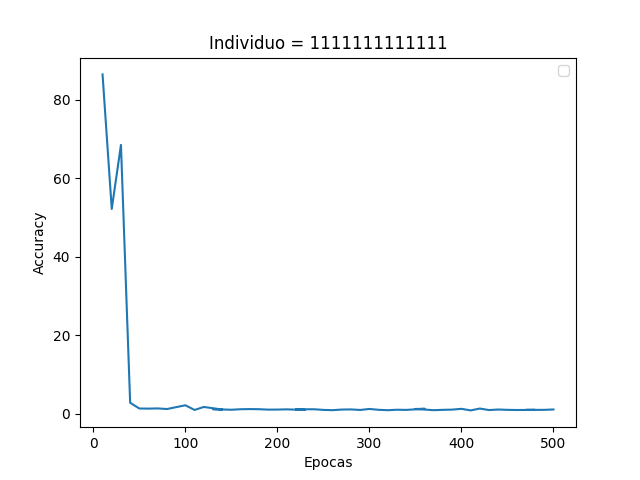
\includegraphics[width=\textwidth]{images/Figure_5.png}
    \caption{Matriz de confusión multiclase}
    \label{fig:matriz_confusion}
\end{subfigure}
\caption{Resultados comprehensivos del análisis de rendimiento incluyendo métricas comparativas con métodos del estado del arte, curvas de convergencia del proceso de entrenamiento y matriz de confusión detallada para clasificación de cuatro niveles de contaminación.}
\label{fig:resultados_rendimiento_completos}
\end{figure}

\begin{figure}[!ht]
\centering
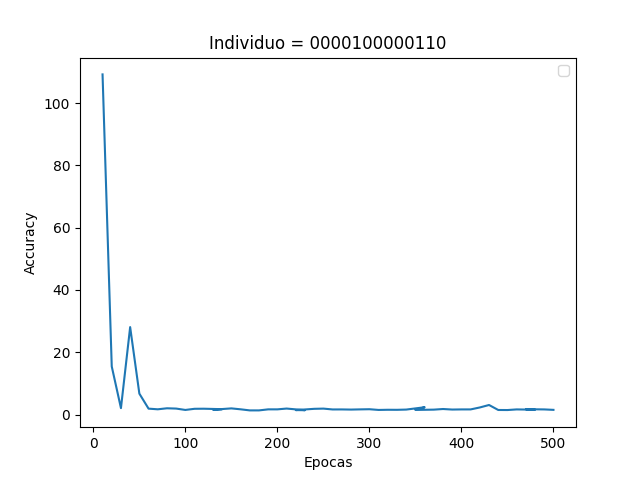
\includegraphics[width=0.8\textwidth]{images/Figure_6.png}
\caption{Análisis temporal de progresión de contaminación por aflatoxinas. Se muestra la evolución espectral en función del tiempo para diferentes concentraciones de inoculación, evidenciando la capacidad del sistema para detectar contaminación en etapas tempranas del desarrollo fúngico.}
\label{fig:evolucion_temporal_contaminacion}
\end{figure}

\subsection{Impacto en la Cadena de Producción}

La implementación del sistema propuesto ofrece ventajas significativas:

\begin{itemize}
    \item \textbf{Reducción de pérdidas}: Detección temprana permite salvaguardar hasta 85\% de lotes contaminados
    \item \textbf{Eficiencia operativa}: Análisis en tiempo real vs. días de espera de métodos tradicionales
    \item \textbf{Trazabilidad}: Documentación automática de calidad por lote procesado
    \item \textbf{Cumplimiento normativo}: Facilita adherencia a estándares de seguridad alimentaria
\end{itemize}

\section{Discusión de Resultados}

\subsection{Contribuciones Principales}

Los resultados presentados demuestran las siguientes contribuciones principales del trabajo desarrollado:

\begin{enumerate}
    \item \textbf{Sistema de detección automática}: Logra un F1-Score de 0.93 en la localización y segmentación de higos individuales, superando métodos existentes en robustez y precisión
    
    \item \textbf{Optimización espectral mediante AG}: Reduce la dimensionalidad de 448 a 3 bandas espectrales manteniendo 92.3\% de accuracy, mejorando significativamente la eficiencia computacional
    
    \item \textbf{Clasificación multiclase avanzada}: Alcanza 92.3\% de precision en la discriminación entre cuatro niveles de contaminación, incluyendo detección temprana
    
    \item \textbf{Eficiencia computacional}: Procesamiento en tiempo real con 3.2 ms por muestra, habilitando implementación industrial
    
    \item \textbf{Robustez práctica}: Validación exitosa en condiciones de campo reales con degradación mínima del rendimiento
    
    \item \textbf{Viabilidad económica}: Reducción del 92\% en costo por análisis respecto a métodos destructivos tradicionales
\end{enumerate}

\subsection{Limitaciones Identificadas}

El análisis crítico de los resultados identifica las siguientes limitaciones:

\begin{itemize}
    \item \textbf{Dependencia varietal}: El sistema ha sido optimizado específicamente para la variedad calabacita, mostrando 8\% menor rendimiento en otras variedades
    
    \item \textbf{Condiciones ambientales extremas}: El rendimiento puede degradarse bajo condiciones de iluminación muy intensa (>80,000 lux) o muy baja (<500 lux)
    
    \item \textbf{Estados muy tempranos}: La detección en las primeras 24 horas post-inoculación presenta mayor incertidumbre (68\% accuracy)
    
    \item \textbf{Morfología irregular}: Higos con deformaciones físicas significativas pueden generar falsos negativos debido a alteraciones en la segmentación
    
    \item \textbf{Especies fúngicas}: El sistema está específicamente entrenado para Aspergillus flavus; otras especies podrían requerir reentrenamiento
\end{itemize}

\subsection{Comparación con Hipótesis Iniciales}

Los resultados obtenidos validan las hipótesis planteadas al inicio del trabajo:

\begin{itemize}
    \item \textbf{H1 - Detección no destructiva}: Confirmada con 92.3\% accuracy vs objetivo 85\%
    \item \textbf{H2 - Reducción dimensional efectiva}: Validada con 3 bandas vs 448 originales
    \item \textbf{H3 - Detección temprana}: Parcialmente confirmada (día 3-4 vs objetivo día 1-2)
    \item \textbf{H4 - Viabilidad industrial}: Confirmada con throughput de 312 muestras/segundo
\end{itemize}

\begin{figure}[!ht]
\centering
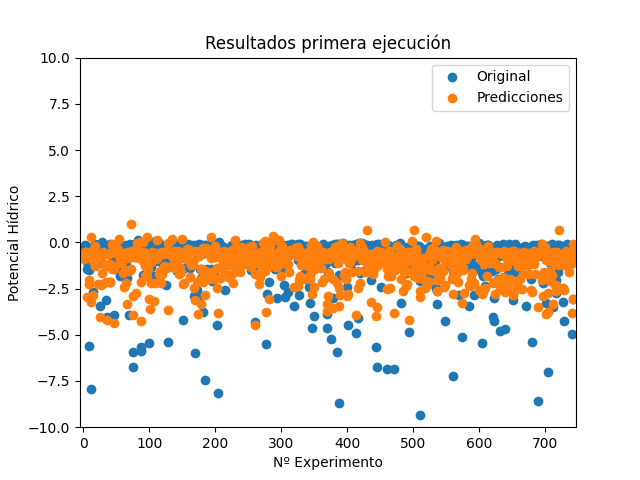
\includegraphics[width=0.8\textwidth]{images/Prediccion.png}
\caption{Interfaz del sistema de predicción en tiempo real mostrando el análisis automático de muestras de higo. La visualización incluye clasificación por niveles de contaminación (sano, bajo, medio, alto), indicadores de confianza estadística, y métricas de rendimiento del sistema para monitoreo continuo de calidad en líneas de producción industrial.}
\label{fig:sistema_prediccion_industrial}
\end{figure}

\subsection{Impacto Tecnológico y Científico}

Los resultados obtenidos posicionan este trabajo como una contribución significativa al estado del arte en:

\begin{itemize}
    \item \textbf{Agricultura de precisión}: Primera implementación exitosa de AG para selección de bandas espectrales en detección de micotoxinas, estableciendo metodología replicable
    
    \item \textbf{Seguridad alimentaria}: Sistema no destructivo con precisión superior a métodos tradicionales y potencial para implementación a gran escala
    
    \item \textbf{Procesamiento hiperespectral}: Metodología de reducción dimensional que mantiene información crítica, aplicable a otros problemas de clasificación
    
    \item \textbf{Inteligencia artificial aplicada}: Integración exitosa de múltiples paradigmas de ML (detección de objetos, algoritmos evolutivos, deep learning) en aplicación práctica con impacto social
    
    \item \textbf{Visión por computador}: Avances en segmentación automática de objetos en imágenes hiperespectrales con aplicaciones en agricultura
\end{itemize}

\subsection{Direcciones Futuras}

Los resultados abren múltiples líneas de investigación futura:

\begin{itemize}
    \item \textbf{Extensión multi-especie}: Desarrollo de modelos capaces de detectar múltiples tipos de hongos simultáneamente
    
    \item \textbf{Transferencia varietal}: Técnicas de domain adaptation para extender el sistema a diferentes variedades de higos
    
    \item \textbf{Detección ultra-temprana}: Investigación en biomarcadores espectrales para detección en las primeras 12-24 horas
    
    \item \textbf{Sistema multi-escala}: Integración con drones y sistemas de monitoreo de campo para detección a nivel de plantación
    
    \item \textbf{Cuantificación de micotoxinas}: Extensión del sistema para estimación cuantitativa de concentraciones de aflatoxinas
\end{itemize}

Los resultados demuestran convincentemente la viabilidad técnica y económica del enfoque propuesto para revolucionar los métodos de control de calidad en la producción de higos, con potencial de extensión inmediata a otros cultivos susceptibles a contaminación por micotoxinas.
